

PLATO is a CTDE method for multi-agent systems with TO and AO, as shown in Figure~\ref{fig:architecture}. PLATO's core novelty is reformulating action selection from fixed-index classification to \emph{content-based pointing}: each agent forms a context vector (query) and selects among the currently available tasks by matching this query against task feature vectors (keys). The policy output size is determined by the current task set, so tasks and agents can appear or disappear without retraining or architectural changes, keeping the policy well-defined as openness changes the environment. %Here, we first present the pointer actor (Section~\ref{actor}), then formalize the observation factorization used by the actor (Section~\ref{factorization}), detail the GNN critic (Section~\ref{critic}), and finally outline the training and complexity involved (Section~\ref{training}).

%OLD - Lengthy
%This section presents \textbf{PLATO}, a CTDE method for multi-agent systems with \emph{agent openness} and \emph{task openness}, where the active agent set and task set vary over time. At timestep $t$, let $N^t$ be the current agent set and $X^t$ be the current task set (Figure~\ref{fig:architecture}). At execution time, each agent $i \in N^t$ applies a shared decentralized policy $\pi_\theta(\cdot \mid o_i^t)$ to select one task from its currently available task-action set. During training, a centralized critic $V_\phi(s^t)$ evaluates the open global state by reasoning over a bipartite agent--task graph from the state. We next formalize the observation factorization used by the actor, then present the pointer actor (Section~\ref{actor}), the GNN critic (Section~\ref{critic}), and the training  (Section~\ref{training}). Note that the novelty of the PLATO approach lies in the pointer mechanism. The pointer actor outputs a policy over a variable-sized action space whose support matches the currently available tasks, and all agents share the same actor parameters, allowing agents and tasks to appear or disappear from the environment without retraining.



%v2
%This section presents \textbf{PLATO}, our approach for learning under openness in multi-agent systems, where both the agent set and the task set may change over time (Figure~\ref{fig:architecture}). First, we refer to the formal open agent--task setting and the TaAgO-MG observation factorization used throughout the method. Next, we introduce the shared pointer-network actor (Section~\ref{actor}), which preprocesses local observations into an agent-context query and a variable-sized set of task keys, and then applies additive cross-attention to produce a categorical policy over the currently available tasks. Then, we present the centralized GNN critic (Section~\ref{critic}), which represents the open global state as a bipartite agent--task graph and computes a state-value estimate via message passing and permutation-invariant pooling. Finally, Algorithm~\ref{alg:plato} describes the end-to-end CTDE training procedure using MAPPO.

%This section presents \textbf{PLATO}, our approach for learning under openness in multi-agent systems, where both the agent set and the task set may change over time. An overview of the complete PLATO architecture is shown in Figure~\ref{fig:architecture}. We describe PLATO beginning with the \textit{shared pointer-network actor} in Section~\ref{actor}, which preprocesses agent and task observations into queries and keys and applies a pointer mechanism to produce an action distribution over a variable available set. The agent set is summarized using permutation-invariant statistics to form a fixed-dimensional query, which conditions task selection on the current team composition and avoids aliasing between different agent sets. The pointer actor outputs a policy over a variable-sized action space whose support matches the currently available tasks, and all agents share the same actor parameters, allowing agents to enter or leave the system without retraining. Next, Section~\ref{critic} introduces the \textit{centralized GNN critic}, which receives the open global state as a bipartite agent--task graph and computes value estimates through relational reasoning during training. Finally, Algorithm~\ref{alg:plato} presents the end-to-end training procedure under the CTDE paradigm using MAPPO.


%TODO subfigure this with an example zero shot showing how the agent graph expands in critic.
\begin{figure}[htbp]
  \centering
  \includegraphics[width=0.5\linewidth]{figs/plato_diagram.png}
  \caption{\small \textbf{PLATO architecture for OASYS.} It uses a pointer actor approach and CTDE training. %The actor factors each agent's local observation into features, summarizes team into a query, embeds each available task into a key, and applies additive cross-attention to produce a categorical policy over the currently available tasks.% During training, the critic represents the global state as a bipartite agent--task graph, performs message passing, pools node embeddings permutation-invariantly, and outputs a scalar state value.
  }
\label{fig:architecture}
\end{figure}



\subsection{Pointer Actor}\label{actor}
The pointer actor is the decentralized policy used at execution time. It supports TO by producing a policy whose support matches the currently available tasks, and supports AO by conditioning decisions on a permutation-invariant summary of the current team. The actor (1) deterministically factors $o_i^t$ into an agent-feature matrix and a task-feature matrix, (2) encodes the current agent set into a fixed-dimensional query, (3) encodes each available task into a key, and (4) applies additive cross-attention to obtain a categorical distribution over the available task-actions. %During training, the pointer actor learns to assign higher attention scores to tasks whose key embeddings yield higher expected returns under the centralized critic \cite{ptr}.%using policy-gradient updates 

This pointing-based design makes PLATO structurally compatible with openness. Standard MARL policies implement fixed-index classification, so the meaning of each output dimension depends on a fixed action roster and often requires padding to a chosen maximum.  PLATO instead applies the same compatibility function to the \emph{current} task keys, so the distribution is defined for any $|X^t|$ and does not depend on task indices. AO is handled by forming $q^t$ from a "team"-based summary, so the same shared policy applies to any subset of agents.  Furthermore,  PLATO processes tasks as a set (no positional indices), summarizes agents, and uses normalized features (e.g., positions and resources as ratios). Hence, task meaning is tied to features and relations, \emph{not to absolute indices or grid-specific coordinates}. This allows PLATO to handle TO.


%This subsection defines the decentralized policy used at execution time. We describe how each agent maps its local observation into (i) a permutation-invariant agent-context query and (ii) a variable-sized set of task keys, and then applies additive cross-attention to produce a categorical policy over the currently available tasks in the decoder.


%We use a shared pointer-network actor inspired by the encoder--decoder structure of pointer networks \cite{ptr}, where an encoder embeds inputs and a decoder selects one element by attending over them using attention scores. The pointer actor is a shared-parameter pointer-network policy that supports \emph{task openness (TO)} and \emph{agent openness (AO)} without requiring fixed upper bounds on \( |X^t| \) or \( |N^t| \). At each timestep, local observations are preprocessed into two representations: an agent encoding that summarizes the current agent composition into a fixed-dimensional, permutation-invariant query, and a task encoding that maps each available task into a latent key. The pointer decoder then applies additive cross-attention between the agent query and the task keys to produce a categorical policy over the currently available tasks. Because decisions are made by content-based attention rather than fixed action indices, the policy naturally adapts to variable task sets under openness.

%\paragraph{Generalization on Unseen Scenarios}
%Because decisions are made in a learned feature space rather than over fixed identities or indices, the policy remains well-defined when agents, tasks, or grid sizes differ from training, and can apply the same selection mechanism whenever the %resulting features fall within the learned representation space.


\subsection{Observation Factorization}\label{factorization}  In TaAgO-MG, the observation of the $i^{\text{th}}$ agent at time $t$, $o_i^t$, is its local view of the global state, $\mathrm{State}^t$, restricted to the current agent set $N^t$ and task set $X^t$ that are visible or relevant to agent $i$.  
The preprocessor factors $o_i$ into an agent-feature matrix $o_N^t \in \mathbb{R}^{|N^t|\times f_N}$ and a task-feature matrix $o_X^t \in \mathbb{R}^{|X^t|\times f_X}$. In these feature matrices, rows correspond to $i$'s observation of tasks and other agents, similar to node factorization for MOHITO's critic graph \cite{anilmohito}. 
% $N^t$ and task nodes $X^t$ used in our TaAgO-MG and in the global graph for the critic.
% As alluded to earlier in Section 3, each task corresponds to exactly one executable task-action available to an agent at time $t$, and we treat each task as one action for the task. 

%\paragraph{Design Rationale}
%Under openness, both the available task set and the agent set vary over time (see \ref{oasys}).
%The policy must therefore select actions from a variable-sized task set while conditioning decisions on the current team composition.
%We address this by using a shared pointer-network policy that performs content-based selection over tasks conditioned on a permutation-invariant summary of the agent set.

\paragraph{Preprocessor.}\label{actor:preprocessor}
This step deterministically splits the local observation into an agent-feature matrix and a task-feature matrix. 
In a TaAgO-MG (Section \ref{sec:open-mas}), $\text{State}^t$ is defined over $(N^t,X^t)$, and each agent observes $o_i^t \in O^t$, a local view of $\text{State}^t$ over the agents and tasks relevant to $i$.
Consider the observations of $i^{th}$ agent $o_i^t \in O^t$. We factor $o_i^t$, by a deterministic Preprocessor, splitting our observation into agent and task features, respectively, $\label{eq:preproc}
    \langle o^t_N \in \mathbb{R}^{|N^t|\times f_N},o^t_X \in \mathbb{R}^{|X^t|\times f_X}\rangle = \textbf{Preprocessor}(o_i^t)$.

\paragraph{Encoder.}\label{actor:encoder}
This step constructs one \emph{query} from the agent set and a variable-sized set of \emph{keys} from the task set. We use MLP encoders since the actor makes a single decision per timestep from fully observable features; sequential decoding is not required.
%Any temporal credit assignment is handled by the environment dynamics and the critic via value estimation.

First, to address AO, we compute four statistics (i.e., mean, variance, minimum, and maximum) over agents in $o^t_N$ to produce a fixed-length vector $d^t$ (Alg.~\ref{alg:plato}, line~10), then encode it as $q^t = \mathrm{MLP}_s(d^t)$ (Alg.~\ref{alg:plato}, line~11). This is \emph{permutation-invariant}: reordering agents does not change $d^t$, see Appendix A.8 for proofs. We use multiple statistics to reduce aliasing, where different agent sets could otherwise produce identical representations. 

Second, to address TO, we construct $|X^t|+1$ keys $K^t$ from $o^t_X$ (Alg.~\ref{alg:plato}, line~12) through the task encoder: one key $k_x^t = \mathrm{MLP}_x(o_x^t)$ per task, plus a \textsc{no-op} key.   In PLATO, we assume one action per task with a persistent \textsc{no-op}, so $a_i^t=\{\textsc{no-op}\}\cup\{\textsf{suppress}(x)\mid x\in X^t\}$. %to isolate open-set selection.
We create the \emph{key}, $k_x^t$, for each task $x$ by embedding $o_x^t$ into a latent space using a task encoder $\mathrm{MLP}_x$. 

%\paragraph{Encoder.}\label{actor:encoder}
%This step produces a fixed-dimensional query summarizing the current agent set and a variable-sized set of keys for the current task set.
%The encoder constructs one \emph{permutation-invariant} \emph{query} from the current agent set and a variable-size set of \emph{keys} from %the current task set for use in our decoder later. The agent query is formed by summarizing $o_N^t$ with multiple statistics,




 %We construct one \emph{query}, $q^t$, from $o^t_N$, through the \textbf{agent encoder}. To address AO, we first summarize $o^t_N$ through element-wise statistics (Alg.~\ref{alg:plato}, line~10). As a critical design element of our Pointer Actor, these team-level statistics serve as a fixed-length permutation-invariant measure of agent composition, $d^t$. We use multiple statistics over ordinary pooling to reduce aliasing, where distinct agent sets would otherwise produce identical pooled summaries.
 %\begin{equation}
%d^t
%  = \big[\;\mu(o^t_N),\;\sigma^2(o^t_N),\;\min(o^t_N),\;\max(o^t_N)\;\big]. \label{eq:agent-stats}
%\end{equation}




\paragraph{Pointing mechanism.}
The agent forms a context query $q^t$ from its local state and the current team summary, and each available task $x\in X^t$ is encoded into a key $k_x^t$ from its features.
The decoder computes a compatibility logit for each $(q^t,k_x^t)$ and normalizes over the current keys, yielding a distribution whose support matches the current task set.



%\paragraph{Pointer Decoder.}\label{actor:decoder}  The \textbf{Pointer Decoder} is a  pointer-network style \cite{ptr} decoder that transforms the \emph{query} and \emph{keys} into a stochastic policy over task-actions conditioned on agent composition, enabling action selection under openness.

\paragraph{Pointer Decoder.}\label{actor:decoder} The Pointer Decoder is a pointer-network style \cite{ptr} module that maps the \emph{query} and \emph{keys} to a stochastic policy over the currently available \emph{task-actions}.  We use one-step, additive attention \cite{bahdanau2014neural} to decode $(q^t,k_x^t)$ to $u_x^t$, a scalar attention score (Alg.~\ref{alg:plato}, line~13), in which, \(\mathbf{W}_K\) and \(\mathbf{W}_q\) are learnable projection matrices, and
\(\mathbf{v}\) is a learnable vector projecting the compatibility space to a scalar score. We then normalize over all attention scores using  SOFTMAX to obtain the policy (Alg.~\ref{alg:plato}, line~14).  Whereas \cite{ptr} uses a sequence-to-sequence setting with autoregressive decoding, PLATO instead uses one-step pointing, since, in MARL, each agent often selects one action per timestep and training uses policy gradients rather than supervised sequence likelihood. 



%\begin{equation}
%u_k^t = \mathbf{v}^\top 
%\tanh\!\left(
%    \mathbf{W}_K\, k_x^t 
%    + 
%    \mathbf{W}_q\, q^t
%\right).
%\end{equation}


%\begin{equation}
%\begin{split}
%    a_x& = \frac{\exp(u_x)}{\sum_{j=1}^{|\mathbf{o}^t_{X}|+1} \exp(u_j)}
%    \\
%    \pi&_\theta(\cdot | \mathbf{s}^t) = \mathrm{Cat}(\mathbf{a}) = \mathrm{Cat}([a_1, \ldots, a_{|\mathbf{o}^t_{X}|+1}])\\
%    a&^t \sim \pi_\theta(\cdot | \mathbf{s}^t).
%\end{split}
%\end{equation}
%Revised equation:
%\begin{equation}
%\begin{split}
%    p_x^t &= \frac{\exp(u_x^t)}
%    {\sum_{j=1}^{|\mathbf X^t| + 1} \exp(u_j^t)}, 
%    \\
%    \pi_\theta(\cdot \mid \mathbf{s}^t) 
%    &= \mathrm{Cat}(\mathbf{p}^t)
%    = \mathrm{Cat}([p_1^t,\ldots,p_{|\mathbf X^t|+1}^t]), 
%    \\
%    a^t &\sim \pi_\theta(\cdot \mid \mathbf{s}^t).
%\end{split}
%\end{equation}

%The support of $\pi$ is $|X^t|+1$, i.e., $a_i^t$ with our assumption that tasks have one associated action, and thus an actor with a dynamic support.




%OLD lengthy
%\paragraph{Handling task openness (TO)}
%At time $t$, the actor embeds each available task into a key $k_x^t$ and produces logits by attending over the current key set. Softmax normalization over the current keys yields a categorical policy with support $|X^t|+1$, so tasks can appear or disappear without padding, upper bounds, or retraining.

%\paragraph{Handling agent openness (AO)}
%All agents share the same policy parameters $\theta$. The current team is summarized into a fixed-dimensional, permutation-invariant query $q^t$ via team statistics. Task selection is conditioned on the current agent composition through the attention compatibility function, which combines each task key with the query $q^t$ to produce selection logits.
%\paragraph{Addressing openness.}  \textbf{TO:} Task openness breaks the standard assumption that the action set is fixed.
%A conventional policy head allocates parameters to a fixed set of action indices, so adding or removing tasks changes what an output dimension means, or requires padding and an a priori maximum number of tasks.
%We therefore need a \emph{content-addressable} policy that can score an arbitrary set of currently available tasks.
%The pointer mechanism provides exactly this: each available task $x\in \bar X_i^t$ is encoded into a key $k_x^t$, and the actor applies the same learned compatibility function
%$f_\theta(q_i^t,k_x^t)$ (via $\mathbf W_q,\mathbf W_K,\mathbf v$) to produce a score for \emph{each} available task.
%Softmax is then applied only over the present keys, yielding a distribution whose support matches $\bar X_i^t$.
%Conceptually, the actor learns a single scoring rule over task \emph{features} (not task IDs), so when tasks appear or disappear the policy %remains well-defined and can generalize by ranking the new set with the same learned rule.

%\textbf{AO:} Agent openness breaks the assumption that the policy can condition on a fixed roster or fixed-size joint state.
%We therefore need a fixed-dimensional, order-invariant representation of the current team that can change in size.
%Permutation-invariant team statistics provide this summary: they map the variable agent set to a fixed-length descriptor that does not depend %on agent ordering.
%Using multiple statistics (mean, variance, min, max) is needed to reduce aliasing that occurs with simple pooling (different team compositions %can share the same mean).
%Embedding these statistics into the query $q_i^t$ lets the shared actor shift its task ranking based on the current team composition, while %keeping one set of parameters $\theta$ that applies to any subset of agents.


%\paragraph{Agent--Task Cross-Attention}
%The pointer actor uses additive cross-attention to compute learned compatibility scores between the current agent context and available tasks in order to select an appropriate task under openness.
%Attention is required because the task set is variable and potentially unbounded, and content-based selection allows the policy output dimension to adapt dynamically at each timestep.
%Task selection is inherently asymmetric: given the current agent composition, the policy must decide which task to execute rather than model relations within the task set.
%Accordingly, the agent set is encoded as a single context query $q^t$, each task is encoded as a key $k_x^t$, and cross-attention evaluates how well each task matches the current agent context, avoiding %fixed action mappings, padding, or predefined upper bounds \cite{ptr}.

%idea is:to calculate how well a task (Key) matches the agent's needs (Query).

%\paragraph{Attention in the Pointer Actor}
%The pointer actor uses attention to compute compatibility scores between an agent-context query and task keys.
%Attention enables content-based selection over a variable-sized set \cite{ptr}, which is required under openness.
%Unlike fixed action mappings, attention allows the policy output dimension to adapt dynamically at each timestep.

 %why we are doing this?reason more 
 %we are asking “given the current team, which task should be chosen.”
 

%\paragraph{Agent--Task Cross-Attention}
%Task selection is inherently asymmetric: given the current agent composition, the policy must select one task from the available task set.
%Accordingly, we encode the agent set into a single query $q^t$ and each task into a key $k_x^t$, and use cross-attention to compute learned compatibility scores that condition task selection on the current team while supporting a variable-sized action space.

\iffalse

%In our design, attention computes compatibility scores between the agents' query (context) $q$ and each encoded key,

\begin{equation}\label{eq:attention}
u^t_k = \mathrm{Attention}(e_k^t, q^t), \quad k \in \{1, \ldots, |X^t|+1\}.
\end{equation}
We use additive (Bahdanau-style) attention \cite{bahdanau2014neural} that projects both keys and query into a shared compatibility space,
\begin{equation}
u_k^t = \mathbf{v}^T \tanh(\mathbf{W}_\mathbf{K} \times e_k^t + \mathbf{W}_q \times  q^t).
\end{equation}
\noindent\textit{where} \(u_k^t\) is the unnormalized attention score for task \(k\) at time \(t\);
\(e_k^t\) is the encoded key from Eq.~\eqref{eq:task-mlp};
\(q^t\) is the agent query from Eq.~\eqref{eq:qt};
\(\mathbf{W}_K\) and \(\mathbf{W}_q\) are learnable projection matrices;
\(\mathbf{v}\) is a learnable vector projecting the compatibility space to a scalar score;
and \(\tanh(\cdot)\) provides nonlinear interaction between the key and query embeddings.


With this we can reason within a fixed-length, learned feature space rather than the unbounded task index space.

\paragraph{\textbf{Policy Generation}}
We normalize the raw attention scores via softmax, then concatenate them to form the distribution of our stochastic policy:
\begin{equation}
\begin{split}
    a_x& = \frac{\exp(u_x)}{\sum_{j=1}^{|\mathbf{o}^t_{X}|+1} \exp(u_j)}
    \\
    \pi&_\theta(\cdot | \mathbf{s}^t) = \mathrm{Cat}(\mathbf{a}) = \mathrm{Cat}([a_1, \ldots, a_{|\mathbf{o}^t_{X}|+1}])\\
    a&^t \sim \pi_\theta(\cdot | \mathbf{s}^t).
\end{split}
\end{equation}
\noindent\textit{where} \(a_x\) is the normalized attention weight for task \(x\);
\(u_x\) is the unnormalized attention score from Eq.~\eqref{eq:key-integrator-eq}; 
\(\pi_\theta(\cdot \mid \mathbf{s}^t)\) is the stochastic policy parameterized by \(\theta\);
\(\mathbf{a} = [a_1, \ldots, a_{|X^t|+1}]\) is the vector of action probabilities;
\(\mathrm{Cat}(\cdot)\) denotes a categorical distribution over available tasks (including no-op);
and \(a^t\) is the sampled action for time \(t\).
The support of this distribution is $A^t_i$ for the $ith$ agent. Attention scores are computed dynamically based on \emph{learned feature similarities}, thus this policy can accommodate unseen task configurations and agent composition without structural change.
\fi

\subsection{GNN Critic} \label{critic}
The critic is centralized during training and estimates $V_\phi(s^t)$ under CTDE. It represents the open global state as a bipartite agent--task graph whose node sets vary with $|N^t|$ and $|X^t|$. Agent and task features are embedded into a shared latent space, message passing propagates relational information across agent--task edges, and pooling yields a fixed-size graph summary that is mapped to a scalar value. This avoids fixed-size concatenation and naturally supports variable numbers of agents and tasks.

%This section describes the centralized critic used by \textbf{PLATO} during training under the CTDE paradigm. The critic estimates the state value $V_\phi(\text{State}^t)$ by representing the global state as a bipartite agent--task graph, where agent nodes and task nodes have distinct semantics and feature spaces. Both node types are encoded into a shared latent space using MLPs, and relational information is propagated through two graph convolutional layers with a residual connection, enabling indirect agent--agent and task--task interactions via agent--task edges. A permutation-invariant mean pooling aggregates the resulting node embeddings into a fixed-size graph representation, which is mapped through a small MLP and a linear value head to produce the scalar state value. Unlike traditional CTDE critics that rely on fixed-size concatenation or padding, this GNN-based design naturally accommodates variable numbers of agents and tasks while preserving relational structure, yielding stable and scalable value estimation under openness.


$\mathcal{G}^t = \langle\mathcal{X}^t, \mathcal{N}^t, \mathcal{E}^t\rangle$
encodes the state, $\text{State}^t$, at time $t$, where
%\begin{itemize}
%\item 
(1) $\mathcal{X}^t \in \mathbb{R}^{|X^t|\times f_X}$ are \emph{task nodes} and contain $f_X$ many features, describing each task at time $t$; (2) $\mathcal{N}^t \in \mathbb{R}^{|N^t|\times f_N}$ are \emph{agent nodes} and contain $f_N$ many features, describing each agent at time $t$; and (3) 
%\item $\mathcal{V} = \mathcal{A} \cup \mathcal{T}$ contains agent nodes and task nodes,  
%\item 
$\mathcal{E}^t$ includes undirected edges between all agent-task pairs which have an action, $\{\langle n,x\rangle | n\in \mathcal{N}^t \text{ and }x\in \mathcal{X}^t\}$.  
%\item $\mathbf{X} \in \mathbb{R}^{|\mathcal{V}| \times d_x}$ holds the initial node features derived from agent observations and task attributes.  
% \end{itemize}

%\begin{figure}
%  \centering
%  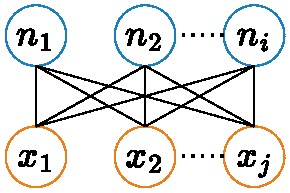
\includegraphics[width=0.6\linewidth]{figs/graph_revised.pdf}
%\caption{\small This global graph represents the environment state for $i$ agents and $j$ tasks.
%Edges encode agents ability to act on tasks.}
%\label{fig:global_graph}
%\end{figure}

%\begin{equation}
%\label{eq:node-embedding}
%\mathbf{h}_0^t = \text{Concat}\left [\text{MLP}_{\mathcal{N}}\left ( \mathcal{N}^t \right ), \text{MLP}_\mathcal{X}\left(\mathcal{X}^t \right ) \right %]\quad \mathbf{h}^t_0\in\mathbb{R}^{|\mathcal{G}^t| f_h},
%\end{equation}
We build a critic network using a GCN \cite{kipf2016semi} to propagate information between agent and task nodes by message passing. First, we use MLP encoders to map $\mathcal{N}^t$ and $\mathcal{X}^t$ into a shared latent space and concatenate them to form $\mathbf{h}_0^t$ (Alg.~\ref{alg:plato}, line~18), where $\mathbf{h}_0^t$  is the embedding of all nodes in $\mathcal{G}^t$ and $f_h$ is the hidden dimension. We then perform message passing (Alg.~\ref{alg:plato}, line~19) with a skip connection \cite{he2016deep} that adds $\mathbf{h}_0^t$ to the final layer output before pooling, preserving individual node features that would otherwise be smoothed out by message passing. We use two layers to allow information to propagate between agents and tasks through the bipartite graph.
Finally, we map the node embeddings to a scalar value by mean pooling over nodes followed by an $\mathrm{MLP}_v$ value head (Alg.~\ref{alg:plato}, lines~\ref{line:critic_pool}--\ref{line:critic_value}).
%\begin{equation}
%    \label{eq:message-passing}
%    \mathbf{h}_1 = \mathrm{ReLU}\left (\frac{\mathbf{h}_0 W_{l}}{\sqrt{|N| \cdot |X|}} \right ) + \mathbf{h}_0,
%\end{equation}


%\begin{equation}
%\label{eq:value-pooling}
%V(\text{State}^t) = MLP_v\left ( \frac{1}{|\mathcal{X}|+|\mathcal{N}|} \sum_{i=1}^{|\mathcal{X}|+|\mathcal{N}|} h^t_{2,i} \right ).
%\end{equation}

\begin{algorithm}[t]
\caption{\textsc{PLATO: Pointer Actor, GNN Critic and training}}
\label{alg:plato}
\small
\begin{algorithmic}[1]
\State \textbf{Inputs:} env $e$, horizon $T$, actor $\pi_\theta$, critic $V_\phi$, initial observation $O^0$
\For{$t=1\ldots T$} 
  \State $a^t_i\sim \textsc{PointerActor}(O_i^t) \quad \forall i \in N^t$
  \State $O^t,\text{State}^t,r^t\gets e(a^t)$
  \State $\hat V^t \gets \textsc{GNNCritic}(\text{State}^t;\phi)$;\; store $(\cdot)$
  \State  compute GAE $\hat A^t$;\; update $\theta$ by PPO-clip;\; update $\phi$ by MSE$(\hat V^t,\hat R^t)$
\EndFor
%\Statex
\Procedure{\textsc{PointerActor}}{$O_i^t$}
  \State $o_N^t,o_X^t\gets \textsc{Preprocessor}(O_i^t)$ 
  
  \State $d^t\!\gets\![\mu,\sigma^2,\min,\max](o^t_{N})$
  %\Comment{Agent Encoding}
  \State $q^t \gets \textsc{MLP}_s(d^t)$
  %\Comment{Task Encoding}
  \State $K^t \gets \{\mathrm{MLP}_x(o) \mid o \in o_X^t\} \cup \{\mathrm{MLP}_x(o_{\textsc{no-op}})\}$ 
  \State $u_x^t\!\gets\!\mathbf{v}^\top\tanh(\mathbf{W}_K k_x^t+\mathbf{W}_q q^t) \quad \forall k_x^t \in K^t$ 
  %\Comment{Pointer Decoding}
  \State  \textbf{return} $\mathrm{Cat}(\mathrm{softmax}([u_x^t]_{x \in X^t \cup \{\textsc{no-op}\}}))$
\EndProcedure
%\Statex
\Procedure{\textsc{GNNCritic}}{$\text{State}^t$} 
  \State form $\mathcal{G}^t=\langle\mathcal{X}^t,\mathcal{N}^t,\mathcal{E}^t\rangle$
  \State $h_0^t \gets \text{Concat}\left [\text{MLP}_{\mathcal{N}}\left ( \mathcal{N}^t \right ), \text{MLP}_\mathcal{X}\left(\mathcal{X}^t \right ) \right ]$
  \State $h^t_l \gets \textsc{GCN}(h^t_{l-1}, \mathcal{E}^t) \quad \text{for each layer }l$
  %\!\gets\!\mathrm{ReLU}(\tilde{D}}^{-\frac12}\tilde{A}}\tilde{D}}^{-\frac12}\mathrm{ReLU}(\tilde{D}}^{-\frac12}\tilde{A}}\tilde{D}}^{-\frac12}e}_gW}^{(1)})W}^{(2)})$

    \State $M^{(L)}\!\gets\!\frac{1}{|\mathcal{N}^t|+|\mathcal{X}^t|}\sum_i(h^t_L + h^t_0)_i$;\; \label{line:critic_pool}
  \State \textbf{return} $V=W_v\,\mathrm{MLP}_v(M^{(L)})+b_v$ \label{line:critic_value}

\EndProcedure

\end{algorithmic}
\end{algorithm}


\iffalse
In CTDE approaches, the critic processes the global state either as a single observation or as a concatenation of agent observations. This assumes a fixed number of agents and tasks, which is incompatible with openness where these sets vary over time. Padding to an upper bound is a possible workaround, but it imposes artificial constraints and defeats the purpose of handling unbounded, variable-sized systems. By instead representing the state as a bipartite graph and applying GNN layers with permutation-invariant pooling, our critic naturally accommodates changing numbers of agents and tasks while preserving relational structure, yielding a flexible and scalable value function.


\subsubsection{\textbf{Global Graph}}\label{global_graph}
This state representation allows our critic to operate on dynamic $N$ and $X$ sets. We represent the global state as a bipartite agent–task graph.
%, as in Figure ~\ref{fig:global_graph}. 
%Nodes are created first (agents, then tasks), and edges are added afterward to connect all agents to all tasks.
 This graph preserves the distinction between agents and tasks while enabling relational reasoning under dynamic, variable-sized configurations. We adopt a bipartite formulation because agents and tasks possess fundamentally different feature spaces and semantic roles. Treating them as a single homogeneous node set would conflate these differences and weaken relational reasoning. By explicitly distinguishing agents from tasks, the critic maintains their identities while still allowing full interaction modeling through graph edges, which is essential for handling openness where both sets vary in size and composition over time.  

At each timestep $t$, the global state $\text{State}^t$ is transformed into a bipartite graph $\mathcal{N}^t \in \mathbb{R}^{|N^t|\times f_N}$, where  
\begin{itemize}
\item $\mathcal{X}^t \in \mathbb{R}^{|X^t|\times f_X}$ are \emph{task nodes} and contain $f_X$ many features, describing each task at time $t$.
\item $\mathcal{N}^t \in \mathbb{R}^{|N^t|\times f_N}$ are \emph{agent nodes} and contain $f_N$ many features, describing each agent at time $t$. 
%\item $\mathcal{V} = \mathcal{A} \cup \mathcal{T}$ contains agent nodes and task nodes,  
\item $\mathcal{E}$ includes fully connected edges among all  agent-task pairs, $\{\langle n,x\rangle | n\in \mathcal{N} \text{ and }x\in \mathcal{X}\}$.  
%\item $\mathbf{X} \in \mathbb{R}^{|\mathcal{V}| \times d_x}$ holds the initial node features derived from agent observations and task attributes.  
\end{itemize}


This construction produces the global graph $\mathcal{G}^t$, which serves as the input to the MLP encoder in the next stage.
Agent nodes $\mathcal{N}$ and task nodes $\mathcal{X}$ are each projected into a shared latent dimension of size $\max(f_X, f_N)$ through learned encoders. Our bipartite edges distinguish agent relationships from task relationships, ensuring that their distinctive features are preserved while still allowing flexible relational reasoning under dynamic and unknown configurations.
%$\mathcal{X}$ and $\mathcal{N}$ are padded with a constant to $\max(f_X, f_N)$.


\subsubsection{\textbf{Node Encoder}}\label{node_encoder}
This component applies MLPs to agent and task node features of the global graph $\mathcal{G}^t$. We use this embedding as a shared latent space of heterogeneous agent and task observations.
%that heterogeneous features are projected into comparable representations for subsequent relational reasoning.
The encoder outputs the initial graph 
embedding matrix,
\begin{equation}
\mathbf{e}_g = \text{Concat}[\text{MLP}_{n}\left ( \mathcal{N} \right ), \text{MLP}_x\left(\mathcal{X} \right )]\quad e_g\in\mathbb{R}^{|\mathcal{G}^t| h}
\end{equation}
where $h$ is the hidden dimension and each row of $\mathbf{e}_g$ corresponds 
to the embedding of a node in $\mathcal{G}^t$.



\subsubsection{\textbf{Graph Convolutional Layers}}\label{gcn}
This component propagates relational information across the bipartite agent–task graph using graph convolutional layers (GCNs) \cite{kipf2016semi}, enabling each node to update its representation based on both local features and the structure of its neighbors. By aggregating information over edges, the critic captures higher-order dependencies among agents and tasks that cannot be expressed by independent node encodings alone. We use two GCN layers, first GCN layer propagates information from agents to tasks via the bipartite edges, and the second propagates back from tasks to agents, enabling indirect agent–agent interaction through two paths ($A\!\to\!T\!\to\!A$) without explicit agent–agent edges. 

\begin{equation} \label{eq:gcn}
\mathbf{H}^{(\ell)} = \text{ReLU}\!\left(\tilde{\mathbf{D}}^{-1/2} \tilde{\mathbf{A}} \tilde{\mathbf{D}}^{-1/2} \mathbf{H}^{(\ell-1)} \mathbf{W}^{(\ell)} \right),
\end{equation}
\noindent where \(\mathbf{H}^{(\ell)}\) is the node-embedding matrix at layer \(\ell\);
\(\mathbf{H}^{(0)}=\mathbf{e}_g\) is the initial node embedding;
\(\tilde{\mathbf{A}}=\mathbf{A}+\mathbf{I}\) is the adjacency with self-loops;
\(\tilde{\mathbf{D}}\) is the degree matrix of \(\tilde{\mathbf{A}}\);
\(\mathbf{W}^{(\ell)}\) is the learnable weight at layer \(\ell\);
and \(\mathrm{ReLU}(\cdot)\) is the elementwise rectifier.
We add a residual connection after the final layer to preserve local features:
\begin{equation}
\mathbf{H}^{(L)} = \mathbf{H}^{(L)} + \mathbf{e}_g.
\end{equation}



\subsubsection{\textbf{Global Pooling and Value Head}} \label{critic_valuehead}
This component aggregates the node embeddings into a fixed-size representation using permutation-invariant mean pooling, ensuring scalability to variable-sized graphs, and then maps this summary through an MLP and a linear head to estimate the centralized state value. By pooling across nodes, the critic preserves global relational information while remaining agnostic to the number and ordering of agents or tasks. This pooling operation is computed as:
\begin{equation}
\mathbf{M}^{(L)} = \frac{1}{|\mathcal{V}|} \sum_{i=1}^{|\mathcal{V}|} \mathbf{H}^{(L)}_i.
\end{equation}
\noindent\textit{where} \(\mathbf{M}^{(L)}\) is the pooled graph representation;
\(\mathbf{H}^{(L)}_i\) is the embedding of node \(i\) from the final GCN layer;
and \(|\mathcal{V}|\) is the total number of nodes (agents and tasks). This pooled vector is then mapped through a MLP to produce estimate state value, $V(\text{State}^t$:
\begin{equation}
\mathbf{V(\text{State}^t}) = \text{MLP}(\mathbf{M}^{(L)}),
\end{equation}
\noindent where \(V(\text{State}^t)\) is the centralized state value estimate at time \(t\);
and \(\mathrm{MLP}(\cdot)\) maps the pooled embedding to a scalar value through a small feedforward network.

\fi

%\paragraph{Activation Functions}
%PLATO uses standard point wise nonlinearities.
%The agent and task encoders use $\mathrm{ReLU}$ \cite{relu_agarap2018deep}, the additive-attention compatibility function uses $\tanh$, and the critic GCN layers use $\mathrm{LeakyReLU}$ \cite{leakyrelu_maas2013rectifier}.



%Mentioned in experiments generalizability section. We may add a much reduced form of this, i.e. move the theoretical comment here, but It need not mention each prop. only the overall theorem proving PLATO is well defined.
% \subsection{Generalizability}\label{sec:generalizability}

% PLATO is structurally well-defined for any number of agents and tasks, without hardcoded count bounds, padding, or configuration changes. We establish this in four propositions following a logical ordering: actor feasibility (Proposition~\ref{prop:welldefined}), ordering invariance under AO (Proposition~\ref{prop:ao}), absence of count-indexed parameters (Proposition~\ref{prop:nobound}), and critic feasibility (Proposition~\ref{prop:critic}). Full permutation-invariance derivations are in Appendix~A.7.



% \paragraph{Scope and limitations.}
% The propositions above establish \emph{structural} generalizability: the computations are always well-formed. They make no claim about \emph{statistical} generalizability — the quality of $\pi_\theta$ and $V_\phi$ on counts far outside the training distribution. A model trained on small systems may still produce unreliable outputs at large scale, even though the forward pass is numerically valid; whether learned representations transfer is an empirical question. A related computational constraint is that the GNN operates on a fully-connected bipartite graph with $|\mathcal{E}^t| = |N^t||X^t|$ edges, scaling as $O(|N^t||X^t|)$ per timestep. At very large scales — say, $|N^t| = |X^t| = 500$, yielding $2.5 \times 10^5$ edges per timestep — this quadratic growth becomes a practical bottleneck; sparse graph approximations could mitigate it but are beyond the scope of the present work. Finally, both the actor and critic assume fixed feature dimensions $f_N$ and $f_X$: if the observation space changes, retraining is required.

\subsection{Training and Complexity}\label{training}

\paragraph{Training.} 

We train PLATO under CTDE using MAPPO \cite{mappo,ppo} with a centralized critic and a single shared policy, while at execution time only the decentralized pointer actor is used. The actor is optimized with the PPO clipped objective \cite{ppo}. The critic uses the standard PPO clipped value regression loss, and we compute advantages with generalized advantage estimation (GAE) \cite{ppo,mappo,gae} (Alg.~\ref{alg:plato}, line 6). All neural components are differentiable in $\theta$ and $\phi$. The preprocessor and team statistics are deterministic tensor operations. Discrete action sampling is handled by the policy-gradient objective and is not differentiated through.  Additional details, including the network architecture and tuned hyperparameters during training, are provided in Appendix A.6. 

%\paragraph{End-to-end differentiability.} 



\paragraph{Computational complexity.}
We treat all fixed hyperparameters ($f_N$, $f_X$, $f_h$, number of GCN layers) as constants and express complexity solely in terms of the quantities that vary under openness: the number of active agents $|N^t|$ and active tasks $|X^t|$.

\paragraph{Actor.}
The preprocessor and team statistics scan $o_N^t$ and $o_X^t$ in $O(|N^t|+|X^t|)$.
The team-statistics step outputs a \emph{fixed}-length descriptor $d^t \in \mathbb{R}^{4f_N}$ regardless of $|N^t|$, so $\mathrm{MLP}_s$ contributes an $O(1)$ constant.
$\mathrm{MLP}_x$ is applied independently to each of the $|X^t|+1$ task features, costing $O(|X^t|)$; because tasks are encoded without shared state, this step parallelizes fully over the task dimension.
One-step additive attention \cite{bahdanau2014neural,ptr} computes a scalar score per key in $O(1)$ and runs over all keys in $O(|X^t|)$; \textsc{Softmax} normalization is likewise $O(|X^t|)$.
The per-agent actor cost is $O(|N^t|+|X^t|)$, and for all $|N^t|$ agents sharing the same policy the per-timestep actor cost is $O(|N^t|(|N^t|+|X^t|))$.

\paragraph{Critic.}
Node encoding via separate MLPs costs $O(|N^t|+|X^t|)$.
The bipartite graph $\mathcal{G}^t$ has $|\mathcal{E}^t|=|N^t||X^t|$ edges; each GCN layer \cite{kipf2016semi} aggregates over $|\mathcal{E}^t|$ edges in $O(|N^t||X^t|)$, which dominates the per-node projection $O(|N^t|+|X^t|)$.
With $L=2$ layers and a residual connection \cite{he2016deep}, total propagation is $O(|N^t||X^t|)$.
Mean pooling and the value head are $O(|N^t|+|X^t|)$ and $O(1)$, respectively.
The critic cost per timestep is therefore $O(|N^t||X^t|)$, which dominates the actor during training.
At execution time the critic is absent, and the cost across all agents reduces to $O(|N^t|(|N^t|+|X^t|))$ per timestep.
Since neither $|N^t|$ nor $|X^t|$ is bounded a priori, PLATO scales continuously to open environments without architectural change.



%\paragraph{End-to-end differentiability.} 



%\paragraph{Computational complexity.}
%For agent $i$, the actor costs $O(|N_i^t|+|X_i^t|)$ for preprocessing and encoders, and $O(|X_i^t|)$ for attention and softmax. The critic builds a graph with $|N^t|+|X^t|$ nodes and $|\mathcal{E}^t|$ edges; %each GCN layer costs $O(|\mathcal{E}^t| f_h)$, and pooling is $O((|N^t|+|X^t|)f_h)$.



%\paragraph{Activation functions.} %went to appendix in network architecture 
%T%he actor and critic use pointwise nonlinearities. We use $\mathrm{ReLU}$ in the MLP encoders, $\tanh$ \cite{relu_agarap2018deep} in the %additive-attention compatibility function, and $\mathrm{LeakyReLU}$\cite{leakyrelu_maas2013rectifier} in the GCN layers.



%\paragraph{End-to-End Differentiability}
%PLATO is fully differentiable with respect to all learnable neural network parameters.
%The agent encoder, task encoder, key integrator, pointer attention module, and decoder consist of affine transformations and standard nonlinear activations.
%The critic network, including node encoders, graph convolution layers, pooling, and value head, is differentiable given the constructed graph input.
%Statistical agent summaries (mean, variance, min, max) are deterministic tensor operations implemented within the neural computation graph.
%Discrete action selection is not part of the learning computation; policy optimization is performed through the differentiable log-likelihood objective.

%\paragraph{Computational Complexity}

%At each timestep, the pointer actor operates on the current agent set \(N^t\) and task set \(X^t\). The preprocessor and agent statistics computation scale linearly as \(O(|N^t|)\), while task encoding scales as \(O(|%X^t|)\). The pointer decoder applies additive cross-attention between the agent query and all task keys, yielding \(O(|X^t|)\) time and space complexity per agent. During training, the centralized critic constructs a bipartite agent--task graph with \(|N^t|+|X^t|\) nodes and \(|N^t||X^t|\) edges; each GCN layer therefore scales as \(O(|N^t||X^t|)\). With a fixed number of GCN layers and constant hidden dimensions, the overall per-timestep training complexity is dominated by the critic, while execution-time complexity remains linear in the number of available tasks.